\documentclass[12pt]{article}

\usepackage{sbc-template}

\usepackage{graphicx,url}

%\usepackage[brazil]{babel}   
\usepackage[latin1]{inputenc}  

     
\sloppy

\title{Graph Database: Neo4J da teoria � pratica. }

\author{Eduardo Pereira da Silva\inst{1}, Iuri Andreazza\inst{1}, Paulo Gr�bin\inst{1}, Talita Audibert\inst{1} }


\address{Universidade do Vale dos Sinos
  (UNISINOS)\\
  S�o Leopoldo -- RS -- Brasil
  \email{\{eduardobursa,iuri.andreazza,plgrabin,tali.audibert\}@gmail.com}
}

\begin{document} 

\maketitle

\begin{abstract}
  This meta-paper describes the style to be used in articles and short papers
  for SBC conferences. For papers in English, you should add just an abstract
  while for the papers in Portuguese, we also ask for an abstract in
  Portuguese (``resumo''). In both cases, abstracts should not have more than
  10 lines and must be in the first page of the paper.
\end{abstract}
     
\begin{resumo} 
	Este artigo gerencia 
\end{resumo}


\section{Introdu��o}\label{sec:intro}


What is a Graph Database?

A Graph Database is not a database to store graphics or images as its name may suggest. It?s a database that uses graph structures such as nodes, properties and edges to represent and store data. In addition, it allows you to represent any kind of data without the limitation of regular databases.

To better understand, let?s talk about each of these structures individually and what they represent:

Node: A node can be used to represent any type of entity that you can think of, be it a business, a blog post, a location, an oil rig, a city, etc. Graph databases don?t care what type of data they?re representing.

Properties: Properties, sometimes called attributes, are named values that relate to nodes. For example, if we take into consideration our City representation of a node, one of the properties would be ?name?, another would be ?population?, and so on.

Edges: Edges, sometimes called Relationships, connect nodes-to-nodes and organize them into arbitrary structures such as a Map, List or a Tree. It?s important to note that when a node is the start node of a relationship, the relationship from that node?s perspective will be an outgoing relationship. And when a node is at the end of a relationship, the relationship from that node?s perspective will be an incoming relationship. Understanding this will make it easier for you to follow the examples.

What can a Graph Database be used for?

There are many scenarios for which one could consider using a Graph Database. Before I list a few examples, as with any architectural and technical decision, you need to analyze all possible solutions. Then, you can select those that are best for you, according to your specifications.

Some of these scenarios include: social networking, fraud detection, people/movie/music recommendation, manufacturing, etc. Using the social networking example, it would be somewhat trivial to do something like ?given the fact that Bob is my friend, give me all friends that are friend?s of friend?s of friend?s of Bob?. This is possible because of the path-finding algorithms involved are easy to implement by traversing through the graph. Imagine doing that through a relational database? A nightmare!

Another advantage when using a Graph database is that you can easily and more naturally model a domain using a whiteboard or a piece of paper. Specifically, nouns that are used become nodes, verbs become relationships, and adjectives and adverbs become properties.

Graph Database Example

Let?s examine the following scenario and how we would structure it using a Graph Database: John is friends with Bob, and Bob is friends with Mark. Visually, this is how we could represent the scenario:



You notice that the visual representation is pretty much how we verbally expressed our scenario. This is a very simple example that we can use to compare the implementation of a traditional SQL database structure versus a Graph database structure:

Traditional SQL



In a traditional SQL structure, each row in the users table represents a user, and each row in the friends table represents a relationship between two users. If we decide to add additional properties to the users table at a later time, we would have to alter the base structure of that table. And if we wanted to add new properties to only a subset of users we would still have to alter the entire users table, or create a new table to accommodate the new values just for the subset of users. Not an ideal scenario when dealing with tens of millions of records.

Graph Database

Graph Database Structure

On the other hand, a Graph database has no set structure or schema for the data, much like a NoSQL database. Now, let?s understand what the graph above is representing: each node represents an entity ? a User in our case; each node contains property values, in this case it?s the User?s name; and each line represents a relationship between the nodes. This is as simple as it gets. And to complement the scenario described in the traditional SQL example, if we did decide to add additional properties to a subset of users, we could easily perform this action on a per-node level instead of a table-wide transaction.


What is Neo4j

Neo4j is ?The World?s Leading Graph Database? according to Neo Technology, the developer behind the project. It?s a commercially supported open-source graph database implemented in Java and some of the key characteristics include:

Data representation using an intuitive graph-oriented model.
Binding for a number of languages, including Ruby, Python and Closure.
Disk-based, native storage manager completely optimized for storing graph structures for maximum performance and scalability.
Massive scalability, it can handle graphs of several billion nodes/relationships/properties on a single machine.
Easy to use and convenient object-oriented API.
Handles large graphs that don?t fit in memory with durability and a fully persistent transactional store.
Powerful traversal framework for high-speed traversals in the node space.
Optimized for highly connected data.
Small footprint, only about 750k jar file.
It provides a REST interface for languages not supported by its bindings.
It?s capable of traversing depths of over 1000 levels at millisecond speeds.
It provides a dual license: open source and commercial.
It integrates seamlessly with Lucene, providing full-text search to nodes and relationships, including phrase queries, wildcard queries, proximity queries, ranked searching, sorting, and more.





\subsection{Organiza��o}\label{sec:org}

Este artigo est� organizado da seguinte maneira, tendo que, na sess�o ~\ref{sec:intro} temos o trecho introdut�rio, 


\section{Conceito}\label{sec:concept}


\section{Abordagem Pr�tica}\label{sec:pratica}


\section{Trabalhos relacionados}\label{sec:rel}


\section{Conclus�o}\label{sec:con}



% 
% \section{General Information}
% 
% \section{First Page} \label{sec:firstpage}
% 
% should be written in boldface and must precede the text.
% 
% \section{CD-ROMs and Printed Proceedings}
% 
% In some conferences, the papers are published on CD-ROM while only the
% abstract is published in the printed Proceedings. In this case, authors are
% invited to prepare two final versions of the paper. One, complete, to be
% published on the CD and the other, containing only the first page, with
% abstract and ``resumo'' (for papers in Portuguese).
% 
% \section{Sections and Paragraphs}
% 
% Section titles must be in boldface, 13pt, flush left. There should be an extra
% 12 pt of space before each title. Section numbering is optional. The first
% paragraph of each section should not be indented, while the first lines of
% subsequent paragraphs should be indented by 1.27 cm.
% 
% \subsection{Subsections}
% 
% The subsection titles must be in boldface, 12pt, flush left.
% 
% \section{Figures and Captions}\label{sec:figs}
% 
% 
% Figure and table captions should be centered if less than one line
% (Figure~\ref{fig:exampleFig1}), otherwise justified and indented by 0.8cm on
% both margins, as shown in Figure~\ref{fig:exampleFig2}. The caption font must
% be Helvetica, 10 point, boldface, with 6 points of space before and after each
% caption.
% 
% \begin{figure}[ht]
% \centering
% 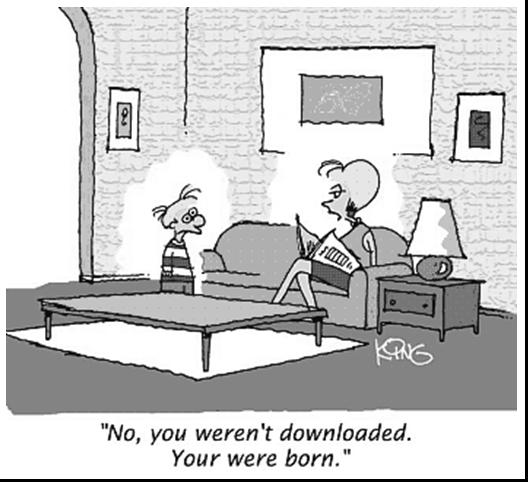
\includegraphics[width=.5\textwidth]{fig1.jpg}
% \caption{A typical figure}
% \label{fig:exampleFig1}
% \end{figure}
% 
% \begin{figure}[ht]
% \centering
% 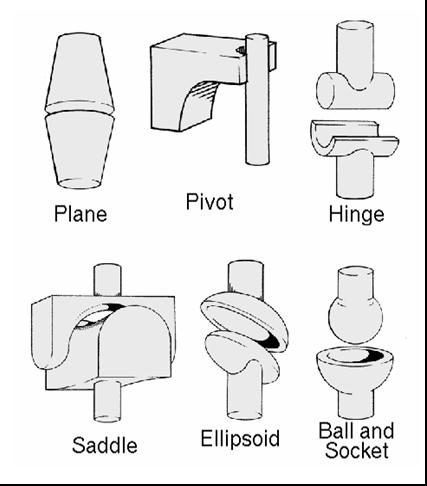
\includegraphics[width=.3\textwidth]{fig2.jpg}
% \caption{This figure is an example of a figure caption taking more than one
%   line and justified considering margins mentioned in Section~\ref{sec:figs}.}
% \label{fig:exampleFig2}
% \end{figure}
% 
% In tables, try to avoid the use of colored or shaded backgrounds, and avoid
% thick, doubled, or unnecessary framing lines. When reporting empirical data,
% do not use more decimal digits than warranted by their precision and
% reproducibility. Table caption must be placed before the table (see Table 1)
% and the font used must also be Helvetica, 10 point, boldface, with 6 points of
% space before and after each caption.
% 
% \begin{table}[ht]
% \centering
% \caption{Variables to be considered on the evaluation of interaction
%   techniques}
% \label{tab:exTable1}
% 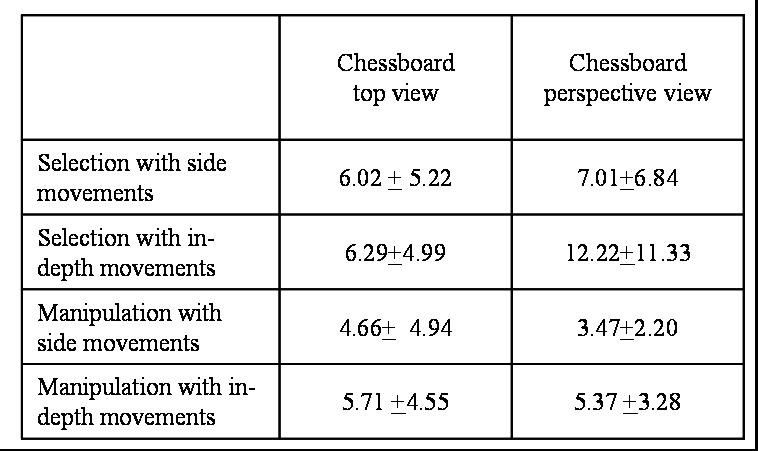
\includegraphics[width=.7\textwidth]{table.jpg}
% \end{table}
% 
% \section{Images}
% 
% All images and illustrations should be in black-and-white, or gray tones,
% excepting for the papers that will be electronically available (on CD-ROMs,
% internet, etc.). The image resolution on paper should be about 600 dpi for
% black-and-white images, and 150-300 dpi for grayscale images.  Do not include
% images with excessive resolution, as they may take hours to print, without any
% visible difference in the result. 

\section{References}

Bibliographic references must be unambiguous and uniform.  We recommend giving
the author names references in brackets, e.g. \cite{knuth:84},
\cite{boulic:91}, and \cite{smith:99}.

The references must be listed using 12 point font size, with 6 points of space
before each reference. The first line of each reference should not be
indented, while the subsequent should be indented by 0.5 cm.

\bibliographystyle{sbc}
\bibliography{sbc-template}

\end{document}
